\documentclass[
  11pt,
  twocolumn,
  a4paper,
%  bibliography=totoc,     % Literatur im Inhaltsverzeichnis
]{article}


% Paket float verbessern
\usepackage{scrhack}

% Warnung, falls nochmal kompiliert werden muss
\usepackage[aux]{rerunfilecheck}

% unverzichtbare Mathe-Befehle
\usepackage{amsmath}
% viele Mathe-Symbole
\usepackage{amssymb}
% Erweiterungen für amsmath
\usepackage{mathtools}
% Fonteinstellungen
\usepackage{fontspec}
% Latin Modern Fonts werden automatisch geladen
% Alternativ zum Beispiel:
%\setromanfont{Libertinus Serif}
%\setsansfont{Libertinus Sans}
%\setmonofont{Libertinus Mono}

% Wenn man andere Schriftarten gesetzt hat,
% sollte man das Seiten-Layout neu berechnen lassen
% \recalctypearea{}
% deutsche Spracheinstellungen
\usepackage{polyglossia}
\setmainlanguage{german}

\usepackage{marvosym}
\usepackage[
  math-style=ISO,    % ┐
  bold-style=ISO,    % │
  sans-style=italic, % │ ISO-Standard folgen
  nabla=upright,     % │
  partial=upright,   % ┘
  warnings-off={           % ┐
    mathtools-colon,       % │ unnötige Warnungen ausschalten
    mathtools-overbracket, % │
  },                       % ┘
]{unicode-math}

% traditionelle Fonts für Mathematik
\setmathfont{Latin Modern Math}
% Alternativ zum Beispiel:
%\setmathfont{Libertinus Math}

\setmathfont{XITS Math}[range={scr, bfscr}]
\setmathfont{XITS Math}[range={cal, bfcal}, StylisticSet=1]

% Zahlen und Einheiten
\usepackage[
  locale=DE,                   % deutsche Einstellungen
  separate-uncertainty=true,   % immer Fehler mit \pm
  per-mode=symbol-or-fraction,
  alsoload=hep,                % / in inline math, fraction in display math
]{siunitx}
\sisetup{math-micro=\text{µ},text-micro=µ}
\DeclareSIUnit\micron{\micro\metre}
\DeclareSIUnit\mrad{\milli\rad}
\DeclareSIUnit\gauss{G}
\DeclareSIUnit\eVperc{\eV\per\clight}
\DeclareSIUnit\nanobarn{\nano\barn}
\DeclareSIUnit\picobarn{\pico\barn}
\DeclareSIUnit\femtobarn{\femto\barn}
\DeclareSIUnit\attobarn{\atto\barn}
\DeclareSIUnit\zeptobarn{\zepto\barn}
\DeclareSIUnit\yoctobarn{\yocto\barn}
\DeclareSIUnit\nb{\nano\barn}
\DeclareSIUnit\pb{\pico\barn}
\DeclareSIUnit\fb{\femto\barn}
\DeclareSIUnit\ab{\atto\barn}
\DeclareSIUnit\zb{\zepto\barn}
\DeclareSIUnit\yb{\yocto\barn}

% chemische Formeln
\usepackage[
  version=4,
  math-greek=default, % ┐ mit unicode-math zusammenarbeiten
  text-greek=default, % ┘
]{mhchem}

% richtige Anführungszeichen
\usepackage[autostyle]{csquotes}

% schöne Brüche im Text
\usepackage{xfrac}

% Standardplatzierung für Floats einstellen
\usepackage{float}
\floatplacement{figure}{htbp}
\floatplacement{table}{htbp}

\RequirePackage{luatex85}
\usepackage[
  locale=DE,
]{siunitx}

\usepackage{tikz}
\usepackage[
  europeanresistors, % follow DIN
  americaninductors, % follow DIN
  siunitx,
]{circuitikz}
\usepackage{stackengine}
\AtBeginDocument{
  \sisetup{
    math-rm=\mathrm,
    math-micro=µ, % AltGr+m = MICRO SIGN, Unicode: U+00B5
  }
}

% Floats innerhalb einer Section halten
\usepackage[
  section, % Floats innerhalb der Section halten
  below,   % unterhalb der Section aber auf der selben Seite ist ok
]{placeins}

% Seite drehen für breite Tabellen: landscape Umgebung
\usepackage{pdflscape}

% Captions schöner machen.
\usepackage[
  labelfont=bf,        % Tabelle x: Abbildung y: ist jetzt fett
  font=small,          % Schrift etwas kleiner als Dokument
  width=0.9\textwidth, % maximale Breite einer Caption schmaler
]{caption}
% subfigure, subtable, subref
\usepackage{subcaption}

% Grafiken können eingebunden werden
\usepackage{graphicx}
% größere Variation von Dateinamen möglich
\usepackage{grffile}

% schöne Tabellen
\usepackage{booktabs}

% Verbesserungen am Schriftbild
\usepackage{microtype}

% Literaturverzeichnis
\usepackage[
  backend=biber,
]{biblatex}
% Quellendatenbank
\addbibresource{lit.bib}
\addbibresource{programme.bib}

% Hyperlinks im Dokument
\usepackage[
  unicode,        % Unicode in PDF-Attributen erlauben
  pdfusetitle,    % Titel, Autoren und Datum als PDF-Attribute
  pdfcreator={},  % ┐ PDF-Attribute säubern
  pdfproducer={}, % ┘
]{hyperref}
% erweiterte Bookmarks im PDF
\usepackage{bookmark}

% Trennung von Wörtern mit Strichen
\usepackage[shortcuts]{extdash}

%Multirow Einbindung
\usepackage{multirow}

%rotating Einbindung
\usepackage{rotating}

%noindent immer da


% \documentclass[11pt, twocolumn, a4paper]{article}

\setlength{\oddsidemargin}{0.0 cm}
\setlength{\evensidemargin}{0.0 cm}
\setlength{\topmargin}{-1cm}
\setlength{\textheight}{24 cm}
\setlength{\textwidth}{16 cm}

\pagestyle{plain}

\setlength{\parindent}{0in}

\begin{document}

\author{Nils Breer}
\date{Technische Universit\"at Dortmund \\
(Dated: August 14, 2020)}

\title{Proceeding to the LHC seminar talk \textit{Update of the $B^0$ \to $K^{*0}$ µ$^{+}$ µ$^{-}$ angular analysis at LHCb experiment} held by Eluned Smith on behalf of the LHC collaboration on 13th of March 2020.}

\maketitle

% meins:

The LHCb collaboration has published new results regarding flavor changing neutral currents based on recent studies for physics beyond standard model. FCNC are very promising decay types since they only occur at loop level and are therefore very sensitive for new physics.
The data from the previous analysis in 2011 and 2012 were expanded by the 2016 data which results in twice the amount of statistics.
With this and a deeper understanding of theoretical uncertainties an angular analysis was performed. The hints on a local tension in $P_5\prime$ were confirmed with this analysis. One of the explanations points to a shift in the wilson coefficient $C_9$.
The most sensitive observables to $C_9$ are the $q^2$ dependence of the forward-backward asymmetry and $P_5\prime$.
The significance of the tension results in $2.7$ - $3.3\sigma$.
The complete set of measurements into the $b \to s \mu^{-} \mu^{+}$ transition performed by various experiments includes the observables $R_K$ and $R_K^{*}$, describing ratios corresponding to $B \to K^{*} ll$ decays involving muons and electrons. This analysis focusses on observables in the $P_i$ and $S_i$ basis and does not include $R_K$ and $R_K^{*}$.
\\~\\
The stated process is of such importance because the
$b \to s \mu \mu$ transition is forbidden at tree level due to FCNC and can only occur at loop order.
Because of that, these processes are much more sensitive to new physics(NP).

\begin{figure}
  \centering
  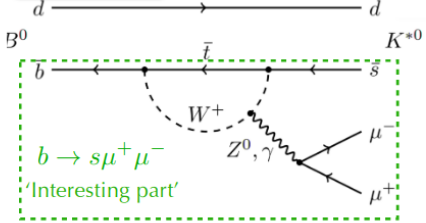
\includegraphics[width=0.4\textwidth]{flavor_plots/sm_process.png}
  \caption{The SM process of $b \to s \mu^{-} \mu^{+}$. \\
          The green box can be described with NP models.}
  \label{fig:sm_process}
\end{figure}

To gather information about short distance NP above the SM energy scale $\mu$, wilson coefficients $C_i(\mu)$ and low-energy QCD Operators $O_i$ are used to describe that.

The wilson coefficients $C_7$, $C_9$ and $C_{10}$ are of great importance since observables like the forward-backward asymmetry and $P_5\prime$ are sensitive for $C_9$ especially.

In an effective theory, $C_9$ and $C_{10}$ are used to describe the contribution from loops, in which electroweak gauge bosons are produced.  wilson coefficient $C_7$ describes the contribution from loopdiagramms which produce photons from the loops.

This can be summarized by an effective hamiltonian
\begin{equation*}
  H_{eff} = - \frac{4 G_f}{\sqrt{2}} \symup{V}_{tb} \symup{V}_{ts}^{*} \sum_i
  C_i(\mu) \cdot O_i(\mu) + \text{h.c.}
\end{equation*}

$G_F$ is Fermi's constant, $\mu$ ist the renormalization scale, $\symup{V}_{tb} \symup{V}_{ts}^{*}$ contains leading flavor factors of the SM which lie in the CKM matrix elements $V_{ij}$.

% \section{angular Analysis}
To measure the decay rate as a function of angles of the decay products, an angular analysis is performed.
This is motivated by the fact, that the $K^{0*}$ is a meson with spin 1 therefore has three polarisation states. This results in a rich angular structure.
The definition of the angular observables $\theta_{k}$, $\theta_{l}$ and $\phi$ is schematically shown in figure \ref{fig:angle_1}

\begin{figure}[htb]
  \centering
  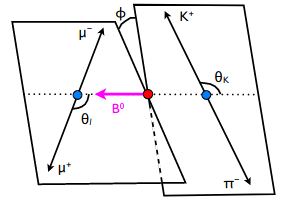
\includegraphics[width=0.4\textwidth]{flavor_plots/angular_describtion.png}
  \caption{image of the angular observables.\cite{Chatrchyan:2013cda}}
  \label{fig:angle_1}
\end{figure}

In this analysis, the forward-backard asymmetry $A_{FB}$, $F_L$ the fraction of the longitudinal polarisation of the $K^{*0}$ and the decay rate of the process $B^0 \to K^{*0} \mu \mu$ was measured. The definition of the angular observables are the following.
$\theta_{l}$ is the angle between the negatively charged lepton and  $\bar{B}$ in the dimuon center of mass system (c.m.s).
$\theta_{k}$ is the angle between the Kaon and the $\bar{B}$ in the $K^{*0}$ c.m.s..
The angle between the $K^{*0}$-plane and the dimuon-plane is defined by the angle $\phi$ in the rest frame of B\cite{Bobeth:2010wg}.

Considering that S-wave contribution, spinless $K^{+}\pi^{-}$ constellations, can pollute the measurement, therefore a parametrization such as $\left(1 - F_S\right)$ for this was taken into account where $(1 -F_S)$ is the S-wave fraction which describes the amount of S-wave contribution.
The interference Amplitude between P-wave and S-wave decays are parametrized by $A_S$.

\begin{align*}
  &\frac{1}{\symup{d}(\Gamma + \bar{\Gamma})/\symup{d}q^2} \frac{\symup{d}^4(\Gamma + \bar{\Gamma})}{\symup{d}q^2\symup{d}\vec{\Omega}} = \frac{9}{32\pi} \\
  &\{ \frac{3}{4}(1 - F_L)\sin^2\theta_K + F_L\cos^2\theta_K \\
  &+ \frac{1}{4}(1 - F_L)\sin^2\theta_K\cos(2\theta_l) \\
  &- F_L\cos^2\theta_K\cos(2\theta_l) \\
  &+ S_3\sin^2\theta_K\sin^2\theta_l\cos(2\phi) \\
  &+ S_4\sin(2\theta_K)\sin(2\theta_l)\cos\phi \\
  &+ S_5\sin(2\theta_K)\sin(\theta_l)\cos\phi \\
  &+ \frac{4}{3}A_{FB}\sin^2\theta_K\cos\theta_l \\
  &+ S_7\sin(2\theta_K)\sin\theta_l\sin\phi \\
  &+ S_8\sin(2\theta_K)\sin(2\theta_l)\sin\phi \\
  &+ S_9\sin^2\theta_K\sin^2\theta_l\sin(2\phi)\}\,.
  \label{eqn:swave}
\end{align*}

The angular description for The $B$ and $\bar{B}$\cite{Aaij:2020nrf} are combined afterwards and expanded into a sum of the angular variables\eqref{eqn:angvar} multiplied with a fitparameter, which are the $A_{FB}$, $F_L$ and $S_i$, which are called CP-averaged observables.
The angular distribution in the $S_i$ basis reads
\begin{equation}
  \frac{\symup{d}^4\Gamma[\bar{B}^0 \to \bar{K}^{0*} \mu^{+} \mu^{-}]}
  {\symup{d}\vec{\Omega}\symup{d}q^2} =
  \frac{9}{32\pi}\sum_i S_i(q_{min}^2, q_{max}^2) f_i(\vec{\Omega})
  \label{eqn:angvar}\,.
\end{equation}

The CP asymmetries need to be analyzed further because NP could contribute differently to CP-conjugated processes.
Afterwards the $S_i$ basis was reparametrised to the $P_i$ basis.
This was done to cancel theoretical uncertainties on the form factors to first order.
The fit to the angular distribution yields seven CP averaged observables including $F_L$.

\begin{align*}
  P_1 &= \frac{2 S_3}{1 - F_L} & P_{4,5,8}\prime &= \frac{S_{4,5,8}}{\sqrt{F_L\left( 1 - F_L \right)}} \\
  P_2 &= \frac{2}{3}\frac{A_{FB}}{1 - F_L} &  P_6\prime &= \frac{S_7}{\sqrt{F_L\left( 1 - F_L \right)}} \\
  P_3 &= \frac{- S_9}{1 - F_L} \\
\end{align*}

Here the angles used for the angular function $f_i(\Omega)$ are $\vec{\Omega} = (\cos\theta_l, \cos\theta_k, \phi)$.
The $S_i$ basis contains the eight angular coefficients which are the combinations of the $K^{0*}$ amplitudes. The forward-backward asymmetry of the dimuon system and teh amount of the longitudinally polarized $K^{0*}$ are also considered for the $S_i$ basis. These amplitudes describe the polarisation states of the Kaon and depend on the wilson coefficients and form factors. An example for the $K^{0*}$ amplitudes is
\begin{align*}
  A_{\bot}^{L(R)} &= \mathcal{N} \sqrt{2\lambda} \{[
  \left( C_9^{\text{eff}} + C_9^{\text{eff}}\prime \right) \mp
  \left( C_{10}^{\text{eff}} + C_{10}^{\text{eff}}\prime \right) \\
  &\frac{V(q^2)}{m_B + m_{K^*}} + \frac{2 m_B}{q^2}
  \left( C_7^{\text{eff}} + C_7^{\text{eff}}\prime \right)T_1(q^2)
  ]\}\,,
\end{align*}
where $T_1(q^2)$ and $V(q^2)$ are form factors and $C_i$ are wilson coefficients.

For this analysis the data sets used are from the years 2011, 2012 and 2016. The data sets from 2011 and 2012 are from run 1.
The 2011 data was taken at a centre of mass energy of $\sqrt{s} = \SI{7}{\tera\electronvolt}$, the 2012 data at $\sqrt{s} = \SI{8}{\tera\electronvolt}$ and the added data set from 2016 was taken at $\sqrt{s} = \SI{13}{\tera\electronvolt}$. Adding the 2016 data also doubled the statistic to around $\SI{4.7}{\femto\barn\tothe{-1}}$.

For the selection of candidates it is required, that the impact parameters of the daughter particles are quite significant since they do not originate from the primary vertex.
% Tracks that come from the primary vertex need to have a very small impact parameter and also a quality vertex is necessary.
That means the track fit $\frac{\chi^2}{dof}$ must be small, where dof are the degrees of freedom.
Also two muon candidates, a kaon and a pion are required.
To suppress peaking background as seen in figure \ref{fig:q2_spec} the particle identification is used.
The FCNC process here is described by $B^0 \to K^{0*}\mu\mu$, but the subprocesses such as $B^0 \to K^{0*}\left(\bar{c}c \to \gamma^{*} \to \mu\mu\right)$ are statistical relevant since they proceed at tree level.
Therefore charmonium resonances pollute the $q^2$ spectrum, especially at the $\symup{J}/\Psi(1S)$ and the $\Psi(2S)$ mass.
Around these peaks a mass-veto region is defined where signal decays are neglected if they fall into the veto region.
Left, in between and on the right of the peaks the signal regions are defined.
Combinatorial background is reduced further using a boosted decision tree (BDT) algorithm. The training uses a cross-validation technique and is performed separately for the Run 1 and 2016 data sets.
Other input variables are the $B^0$ decay time, vertex-fit quality, momentum and transverse momentum of $B^0$ candidate, $\theta_{\text{DIRA}}$ as well as particle identification from the RICH detector.
$\theta_{\text{DIRA}}$ describes the opening angle between the reconstructed $B^0$ momentum and the vector connecting the reconstructed $B^0$ decay vertex to the primary vertex.
The classifier is trained on $B \to J/\Psi K^{0*}$ candidates as signal. The background consists of candidates from the data sidebands $m(B \to K^{+} \pi^{-} \mu^{+} \mu^{-}) \in[5350 \text{MeV}, 7000 \text{MeV}]$.

\begin{figure}[htb]
  \centering
  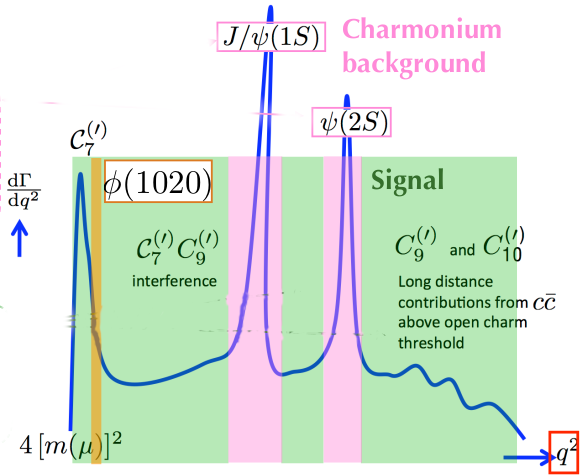
\includegraphics[width=0.4\textwidth]{flavor_plots/regionsq2.png}
  \caption{spectrum in $q^2$ for the \\
  lepton pair in Kll branching fraction\cite{Blake:2017wjz}.}
  \label{fig:q2_spec}
\end{figure}

For the full fit model the shape of the invariant mass plots are used to determine the amount of signal and background in the data.
\begin{equation*}
  \symup{PDF}_{total} = f_{sig}\symup{PDF}_{sig}(\vec{\Omega}, m) +
  (1 - f_{sig})\symup{PDF}_{bkg}(\vec{\Omega}, m)
\end{equation*}

The PDF function can be separated into an angular part and $q^2$.
After that a maximum likelihood fit is performed.
The massive part of the signal PDF is a gaussian function with a radiative tail and the background PDF results in an exponential function.

Because the angular and the $q^2$ dependencies factorize
\begin{align*}
  \symup{PDF}_{sig}(\vec{\Omega}, m) &= \symup{PDF}_{sig}(\vec{\Omega}) \times \symup{PDF}_{sig}(m) \\
  \symup{PDF}_{bkg}(\vec{\Omega}, m) &= \symup{PDF}_{bkg}(\vec{\Omega}) \times \symup{PDF}_{bkg}(m)
\end{align*}
the angular part of the signal PDF from Run 1 and the data from 2016 are shared in the analysis to perform a simultaneous fit $\sum_i S_{i, q_{bin}^2} f_i(\Omega)$. This is possible since only the mass shape is shared. Because the conditions in the 2016 data sample differs from Run 1 data, every other part is different.

The efficiency needs a correction since it's behavior is not flat.
Legendre polynomials are used for the dimuon mass and the three angles which results in a 4D formula. The correlation between the observables forbids the factorization of the 4D function to 1D functions.

The dominant systematic uncertainties are acceptance variations with $q^2$, peaking backgrounds and bias corrections as seen in figure \ref{fig:q2_spec}.
Bias relates to the S-wave contribution $F_S$. If it is small, the angular spectrum is biased towards the P-wave. If $F_S \approx 1$, it is biased towards the S-wave.

With the datasets from Run 1 and 2016 combined a significance of $\SI{2.5}{\sigma}$ in the $q^2 \in [4.0, 6.0] \frac{\symup{GeV}^2}{c^4}$ bin was yieled.
For the $q^2 \in [6.0, 8.0] \frac{\symup{GeV}^2}{c^4}$ bin a significance of $\SI{2.9}{\sigma}$ was yielded.
A local tension in figure \ref{fig:p5_after} was reduced in comparison to figure \ref{fig:p5normal} for both data sets combined.
The global significance is obtained by fitting all observables of the $S_i$ basis to the complete set of CP-averaged observables. The wilson coefficients and all bins in $q^2$ need to be extracted.
The theory uncertainty regarding form factors and parametrisation of sub-leading corrections have decreased from previous publications.

\begin{figure}[htb]
  \centering
  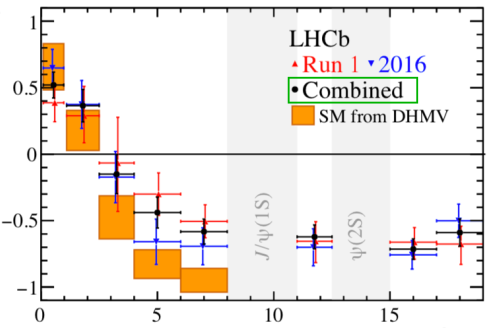
\includegraphics[width=0.4\textwidth]{flavor_plots/p5_tension_after.png}
  \caption{local tension in $P_5\prime$ with combined data.}
  \label{fig:p5normal}
\end{figure}
\begin{figure}[htb]
  \centering
  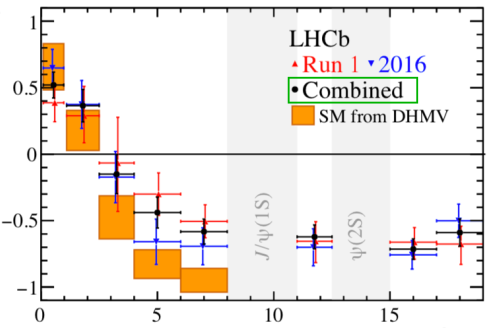
\includegraphics[width=0.4\textwidth]{flavor_plots/p5_tension_after.png}
  \caption{local tension in $P_5\prime$ with combined data.}
  \label{fig:p5_after}
\end{figure}

A variation in the real part of $C_9$ and $C_{10}$ lead to a measureable shift in the wilson coefficients $C_9$ and $C_{10}$, also in agreement to Run 1 as seen in figure \ref{fig:c9c10}.
When only varying $C_9$ the preferred shift can be seen in figure \ref{fig:shift_min}.
It occurs that the 2016 analysis and Run 1 show similar results.
The combination of Run 1 and 2016 yielded, when including the bin
$q^2 \in [6.0, 8.0]\text{GeV}/c^4$, a significance of $\SI{3.3}{\sigma}$ and $\SI{2.4}{\sigma}$ when excluded.
\begin{figure}
  \centering
  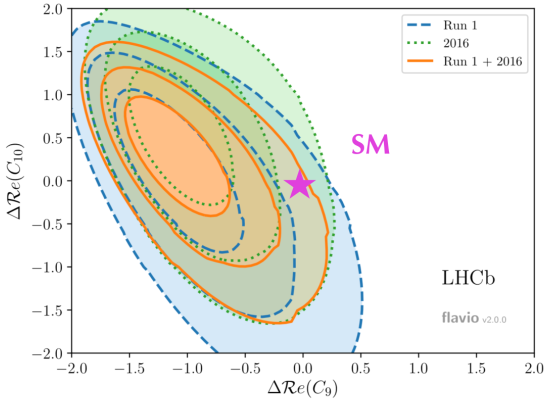
\includegraphics[width=0.4\textwidth]{flavor_plots/shiftc9c10.png}
  \caption{Shift in $C_9$ and $C_{10}$ compared to SM.}
  \label{fig:c9c10}
\end{figure}

In figure \ref{fig:shift} the angular observable $P_5\prime$ as a function of $q^2$ for the SM prediction and the theory prediction with preferred wilson coefficents is shown. It can be seen, that a shift closes the gap between both predictions.
\begin{figure}
  \centering
  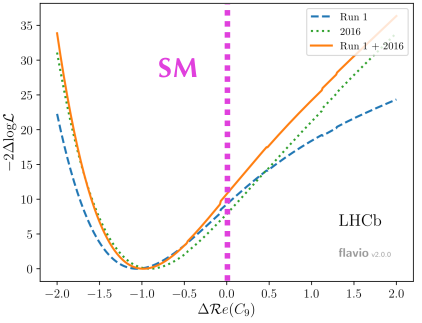
\includegraphics[width=0.4\textwidth]{flavor_plots/shift_min.png}
  \caption{shift in the real part of $C_9$ \\
  yielded from the analysis.}
  \label{fig:shift_min}
\end{figure}
\begin{figure}
  \centering
  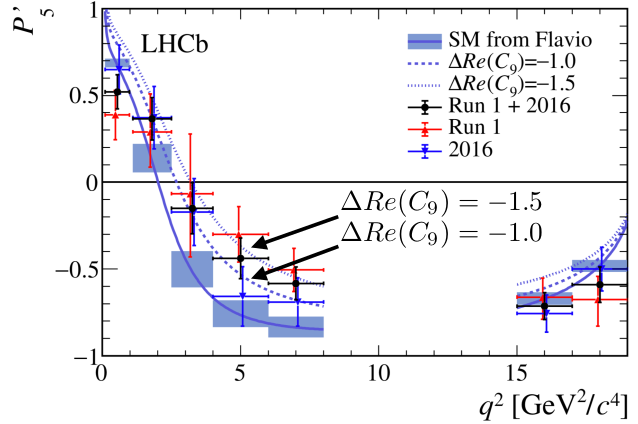
\includegraphics[width=0.4\textwidth]{flavor_plots/shift.png}
  \caption{angular observable $P_5\prime$.}
  \label{fig:shift}
\end{figure}

With that being said, the results presented in the seminar emphasize the overall tension proposed in Run 1 data from previous measurements.
The higher overall tension does not confirm new physics but only hint at it. Different measurements at different scales could yield a deeper understanding an a more precise measurement which might confirm the hints. Further studies in $b \to s$ transitions such as $b \to s \gamma$ could contribute to the analysis\cite{semilep}.
In order to study new physics at higher scales, an angular analysis is important since the optimised basis reduce the theoretical uncertainties from form factors.

\printbibliography{}
\end{document}
